
\section{Comunicación y Animación con Python}

\begin{frame}{Integración completa en Simulink}
  \centering
  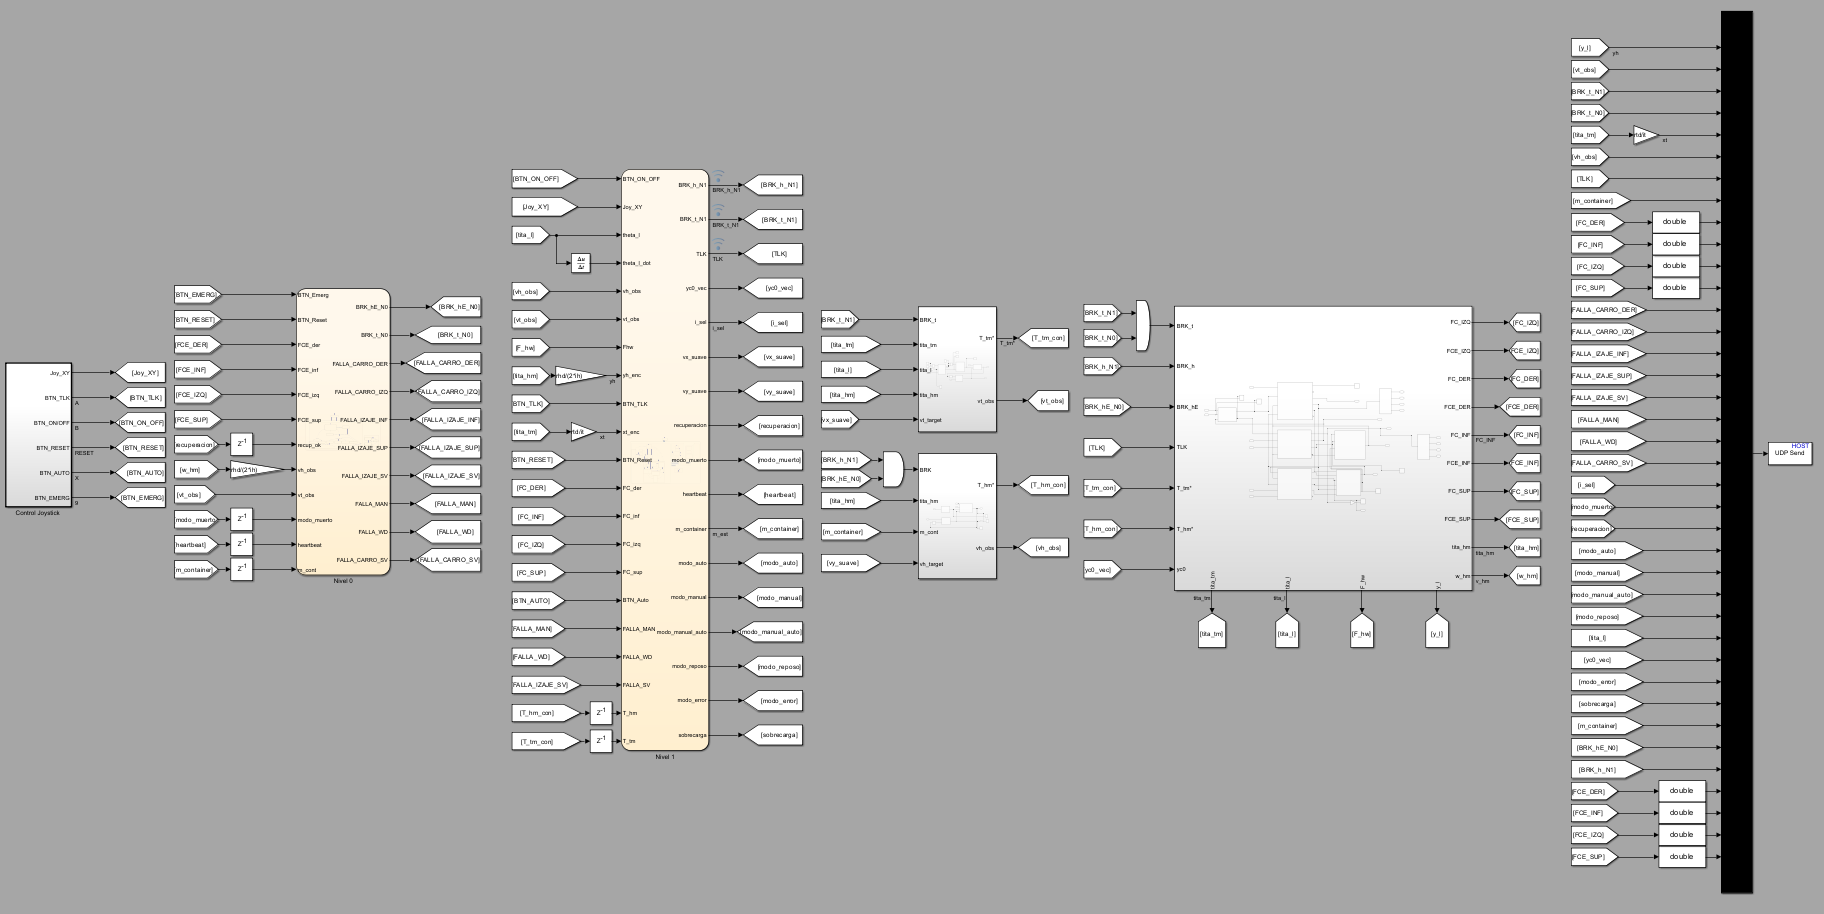
\includegraphics[width=0.95\textwidth]{simulacion/planta_completa.png}
  
  \vspace{0.2cm}
  Planta física + Nivel 2 (control) + Nivel 1 (supervisor) + Nivel 0 (protección) + UDP
\end{frame}

\begin{frame}{Comunicación UDP: Simulink Python}
  \centering
  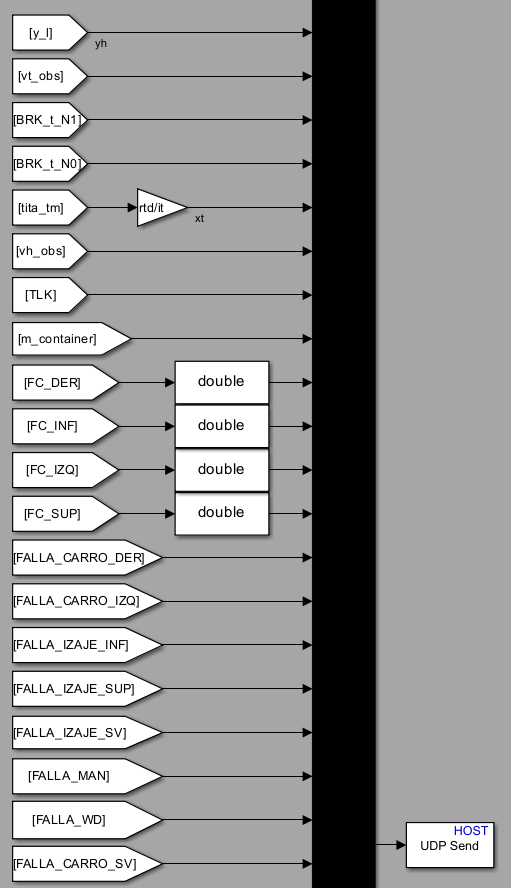
\includegraphics[width=0.32\textwidth]{simulacion/sim_udp.png}
  \hspace{0.3cm}
  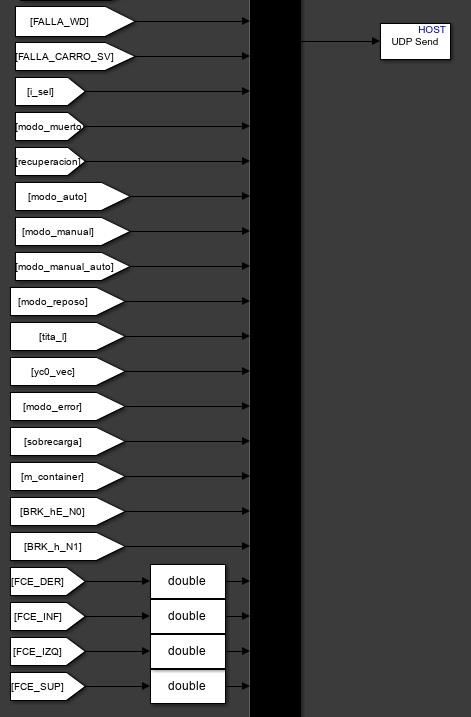
\includegraphics[width=0.32\textwidth]{simulacion/sim_udp2.png}
  
  \vspace{0.2cm}
  Estados de la planta (posiciones, velocidades, sensores) Visualización web en tiempo real
\end{frame}

\begin{frame}{Modo manual}
  \centering
  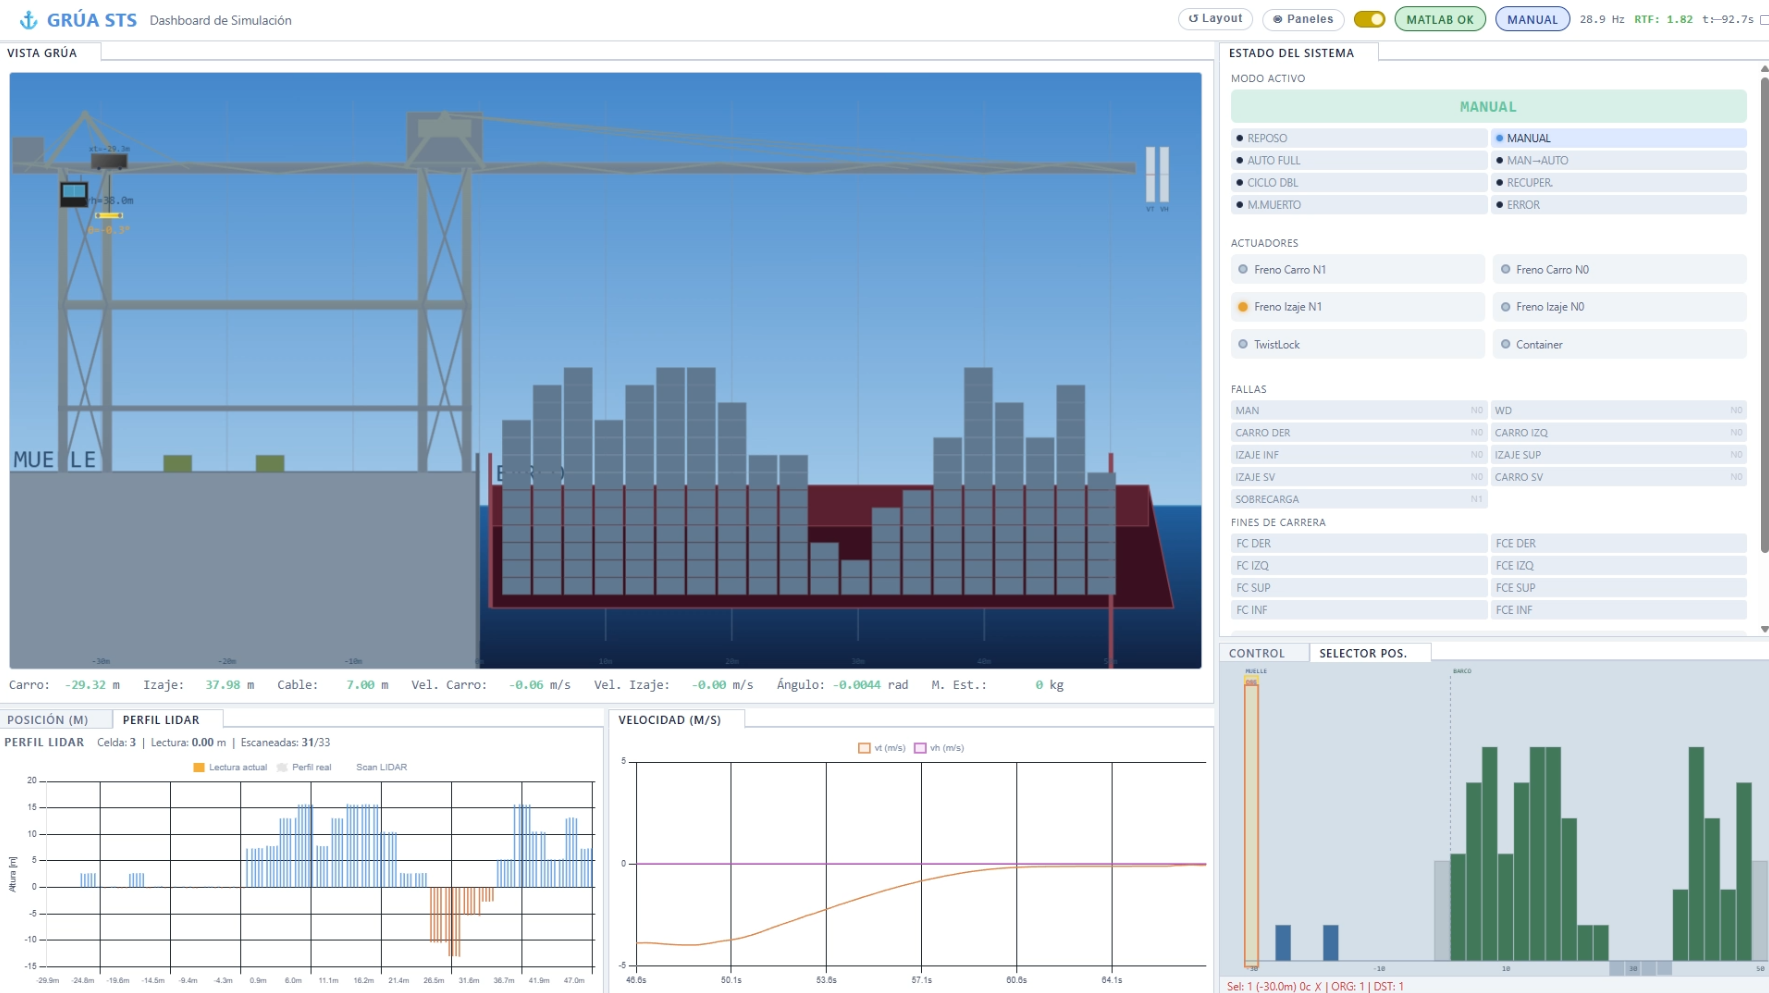
\includegraphics[width=\textwidth]{simulacion/sim_manual.png}
  
  Control del operador por joystick: traslación y elevación de la carga
\end{frame}

\begin{frame}{Modo automático: seguimiento de trayectoria}
  \centering
  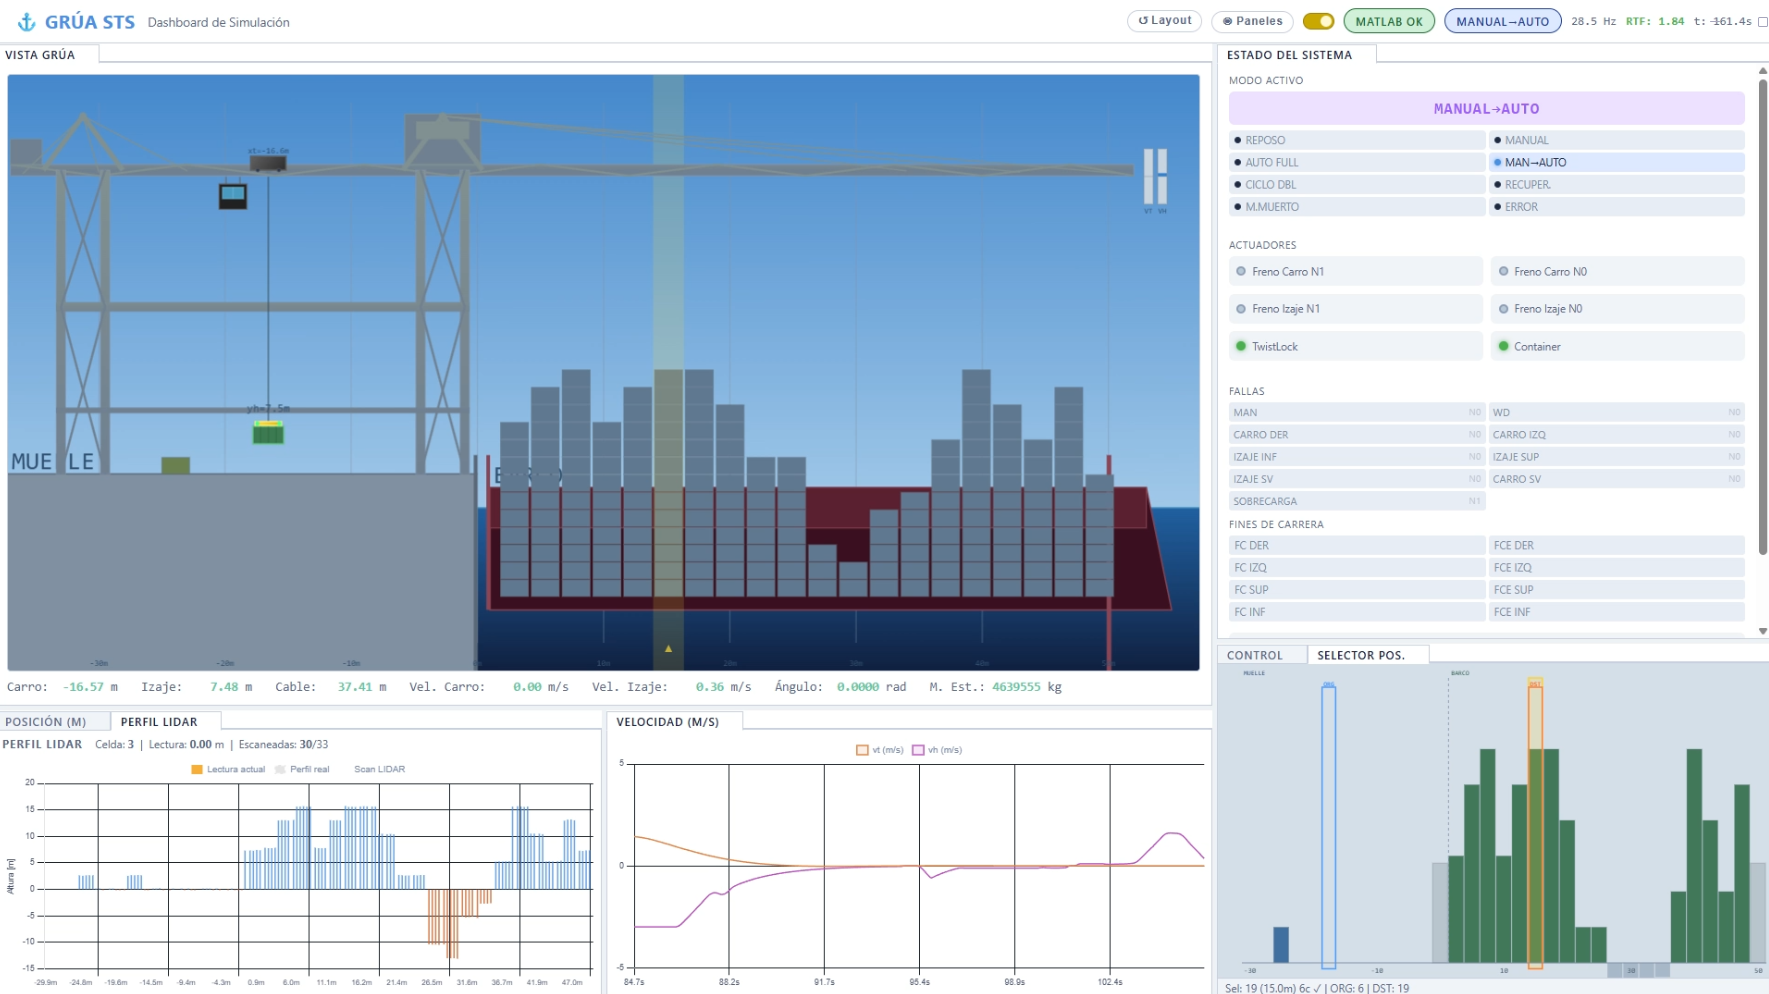
\includegraphics[width=\textwidth]{simulacion/sim_auto.png}
  
  Ejecución automática de la secuencia de operación sin intervención manual
\end{frame}

\begin{frame}{Liberación de la carga}
  \centering
  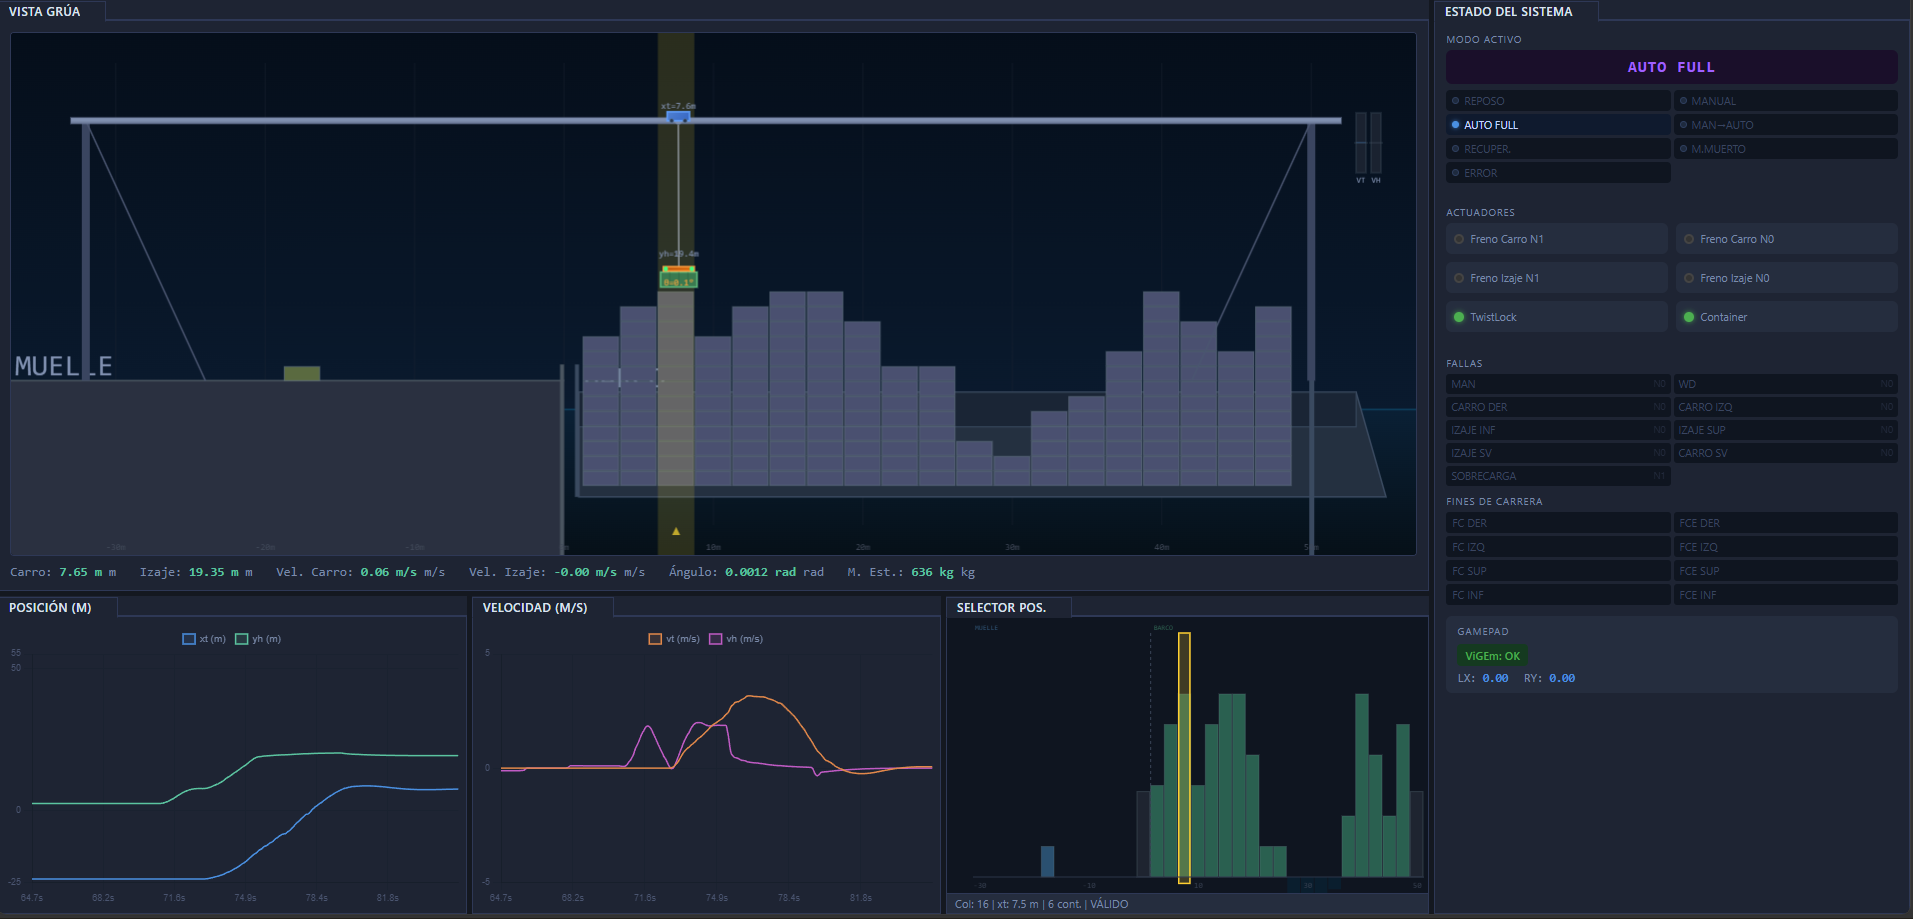
\includegraphics[width=\textwidth]{simulacion/sim_auto_leave.png}
  
  Desenganche de twistlocks y apoyado de la carga en la pila
\end{frame}

\begin{frame}{Estado de error}
  \centering
  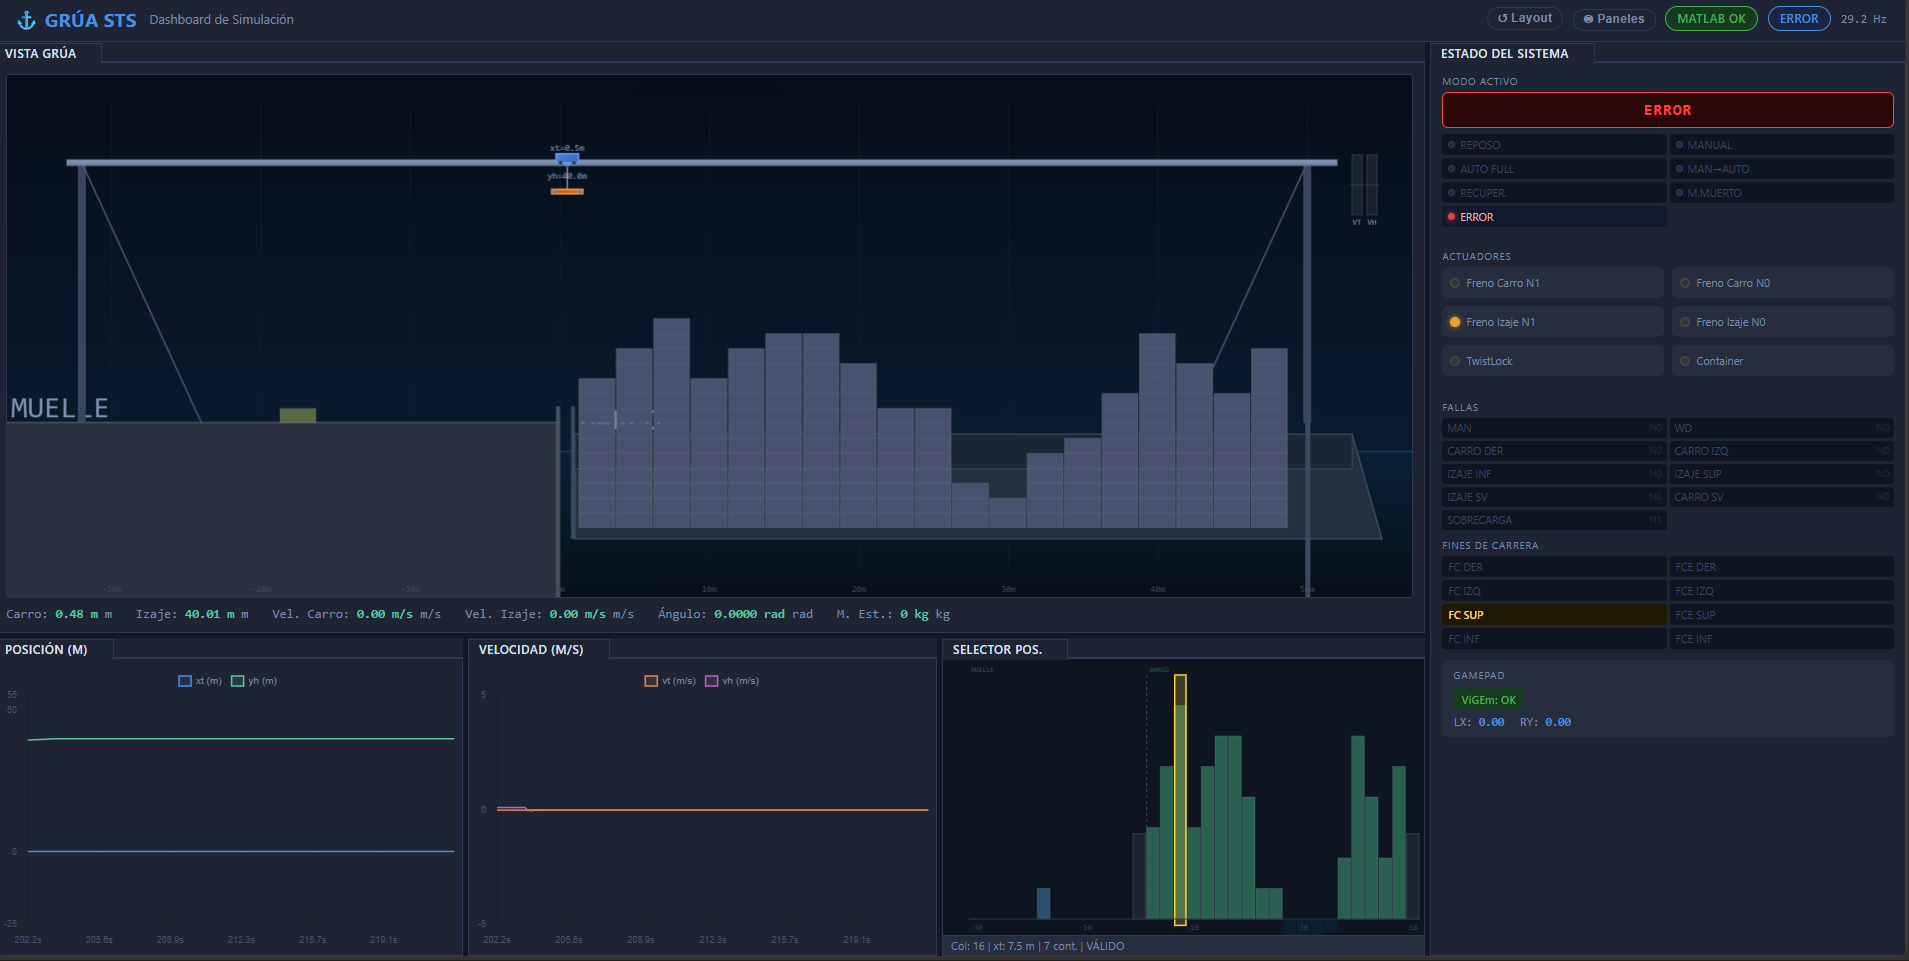
\includegraphics[width=\textwidth]{simulacion/sim_error.png}
  
  Detección de anomalía, aplicación de frenos, indicación de estado de error
\end{frame}
